%%%%%%%%%%%%%%%%%%%%%%%%%%%%%%%%%%%%%%%%%%%%%%%%%%%%%%%%%%%%%%%%%%%%%%
% Overleaf (WriteLaTeX) Example: Molecular Chemistry Presentation
%
% Source: http://www.overleaf.com
%
% In these slides we show how Overleaf can be used with standard 
% chemistry packages to easily create professional presentations.
% 
% Feel free to distribute this example, but please keep the referral
% to overleaf.com
% 
%%%%%%%%%%%%%%%%%%%%%%%%%%%%%%%%%%%%%%%%%%%%%%%%%%%%%%%%%%%%%%%%%%%%%%

\documentclass{beamer}

\mode<presentation>
{
  \usetheme{Madrid}       % or try default, Darmstadt, Warsaw, ...
  \usecolortheme{default} % or try albatross, beaver, crane, ...
  \usefonttheme{default}    % or try default, structurebold, ...
  \setbeamertemplate{navigation symbols}{}
  \setbeamertemplate{caption}[numbered]
} 

\usepackage[english]{babel}
\usepackage[utf8x]{inputenc}
\usepackage{graphicx}
\usepackage{hyperref}
  \hypersetup{colorlinks=true}
  \hypersetup{urlcolor=blue}
  \hypersetup{linkcolor = .}
\usepackage{xcolor}
\usepackage{siunitx}
  \sisetup{separate-uncertainty = true}
\usepackage{physics}
\usepackage[font=small,labelfont=bf]{caption}
\usepackage{subcaption}
\usepackage[en-GB]{datetime2}
\usepackage{overpic}
\usepackage{feynmp}
\DeclareGraphicsRule{*}{mps}{*}{}
\usepackage{scalerel}
\newcommand{\mylbrace}[2]{\vspace{#2pt}\hspace{6pt}\scaleleftright[\dimexpr5pt+#1\dimexpr0.06pt]{\lbrace}{\rule[\dimexpr2pt-#1\dimexpr0.5pt]{-4pt}{#1pt}}{.}}
\newcommand{\myrbrace}[2]{\vspace{#2pt}\scaleleftright[\dimexpr5pt+#1\dimexpr0.06pt]{.}{\rule[\dimexpr2pt-#1\dimexpr0.5pt]{-4pt}{#1pt}}{\rbrace}\hspace{6pt}}

% Here's where the presentation starts, with the info for the title slide
\title[$K^+K^-\pi^+\pi^-$]{\texorpdfstring{$D\to K^+K^-\pi^+\pi^-$}{K+K-pi+pi-} analysis at LHCb and BESIII}

\author{Martin Tat}
\institute{Oxford LHCb}
\date{21st February 2022}

\titlegraphic{
\includegraphics[height = 2cm]{lhcb.jpg}\hspace{1cm}~%
              
\includegraphics[height = 2cm]{OxfordLogo.pdf}\hspace{1cm}~%
              
\includegraphics[height = 2cm]{bes3.jpg}}

\begin{document}

\begin{frame}
  \titlepage
\end{frame}

% These three lines create an automatically generated table of contents.
\begin{frame}{Outline}
  \tableofcontents
\end{frame}

\section{LHCb}

\begin{frame}{$B^\pm\to(K^+K^-\pi^+\pi^-)_Dh^\pm$ GGSZ+GLW analysis at LHCb}
  \begin{center}
    {\huge $B^\pm\to(K^+K^-\pi^+\pi^-)_Dh^\pm$ \\~\\GGSZ+GLW analysis at LHCb}
  \end{center}
\end{frame}

\subsection{Summary of LHCb analysis status}

\begin{frame}{Summary of LHCb analysis status}
  \begin{itemize}
    \setlength\itemsep{0.5em}
    \item{Previously on $\gamma$ measurement in $B^\pm\to Dh^\pm$, $D\to K^+K^-\pi^+\pi^-$:}
    \begin{enumerate}
      \setlength\itemsep{0.5em}
      \item{Model-independent binned GGSZ and inclusive GLW analysis}
      \item{Initial ANA note draft circulated in November}
      \begin{itemize}
        \item{First round of comments received and replies have been sent back}
        \item{No further comments from 2/3 reviewers}
        \item{Still waiting for the last reply}
      \end{itemize}
      \item{All systematics studies finished}
      \item{Potential problem: $s_i$ sign might be wrong}
    \end{enumerate}
  \end{itemize}
  \begin{figure}
    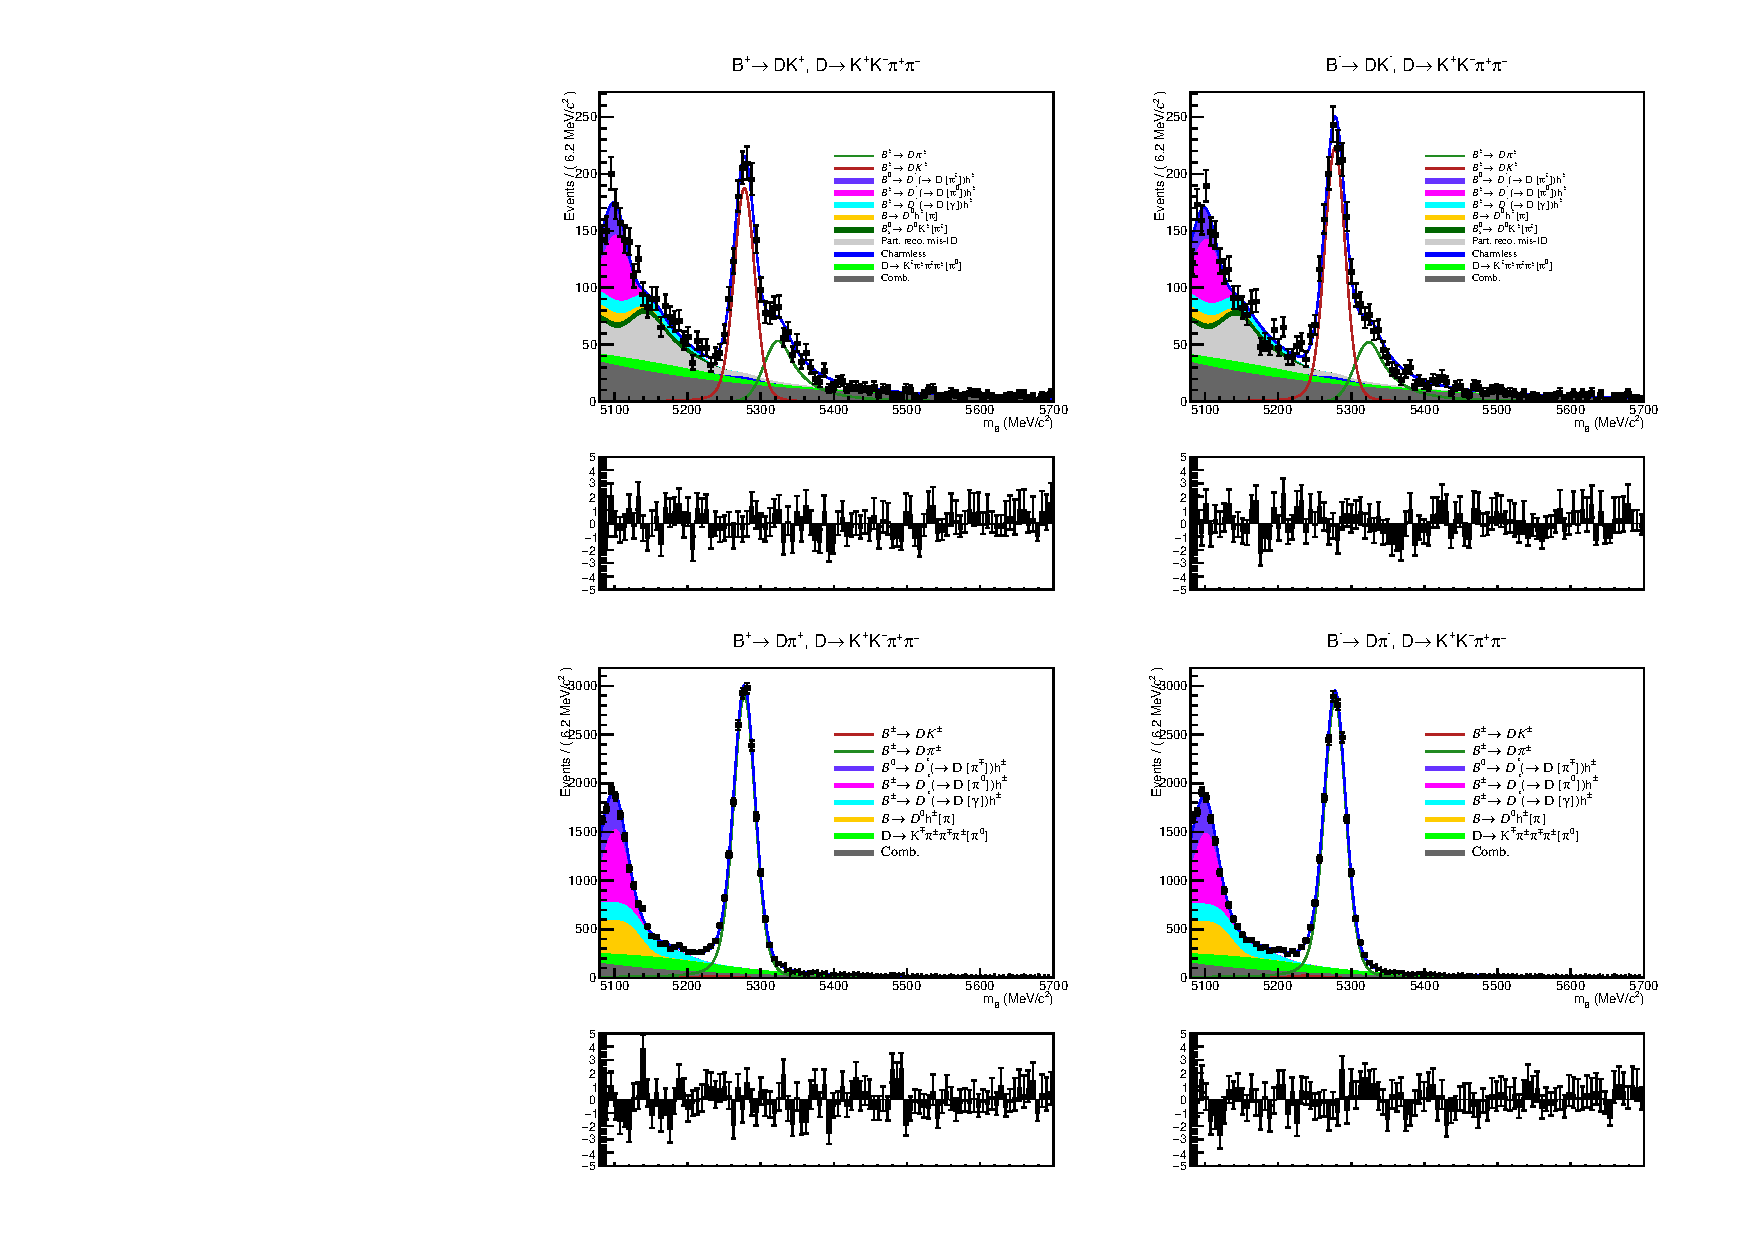
\includegraphics[width = 0.85\textwidth, trim = {0 12.8cm 0 0}, clip]{Plots/d2kkpipi_fiveL_allDP_GLW.pdf}
  \end{figure}
\end{frame}

\begin{frame}{$s_i$ sign problem}
  \begin{itemize}
    \setlength\itemsep{0.5em}
    \item{Amplitude model gives us: $A(\Phi) = \sum_ka_kS_k(\Phi)$}
    \item{Flavour-tagged LHCb data measures: $\abs{A(\Phi)}^2$}
    \item{\underline{Cannot} measure absolute sign of $a_k$ phase}
  \end{itemize}
  \vspace{0.4cm}
  \begin{tabular}{l|c|c}
    Resonance                           & LHCb model phase ($\si{\radian}$) & CLEO model ($\si{\radian}$) \\
    \hline
    $D^0\to[\phi(1020)\rho^0]_{L = 0}$  & $0$ (fixed)                       & $0$ (fixed) \\
    $D^0\to K_1(1400)^+K^-$             & $1.05$                            & $-1.79$ \\
    $D^0\to K_1(1270)^+K^-$             & $2.02$                            & $-2.56$ \\
    \hline
  \end{tabular}
  \vspace{0.4cm}
  \begin{itemize}
    \setlength\itemsep{0.5em}
    \item{BESIII data needed to determine this sign!}
    \item{Reconstruct $KK\pi\pi$ vs $K_{S,L}\pi\pi$ double tags:}
  \end{itemize}
  \begin{center}
    $M_{i, j}\propto\big(K_iK^\prime_{-j} + K_{-i}K^\prime_j - 2\sqrt{K_iK_{-i}K^\prime_jK^\prime_{-j}}(c_ic^\prime_j + s_is^\prime_j)\big)$
  \end{center}
\end{frame}

\section{BESIII}

\begin{frame}{$D\to K^+K^-\pi^+\pi^-$ strong-phase analysis as BESIII}
  \begin{center}
    {\huge $D\to K^+K^-\pi^+\pi^-$ \\~\\strong-phase analysis as BESIII}
  \end{center}
\end{frame}

\subsection{Previously: Measurement of CP even fraction \texorpdfstring{$F_+$}{F+}}

\begin{frame}{Previously: Measurement of CP even fraction $F_+$}
  \begin{itemize}
    \item{BESIII: $e^+e^-$ collider at $\psi(3770)\to D^0\bar{D^0}$ threshold}
    \item{Reconstruct signal mode $D\to KK\pi\pi$ and a tag mode $D\to f$}
    \item{Signal mode is \underline{quantum correlated} with tag mode}
    \item{Measure BF with CP even/odd tags to determine $F_+$}
  \end{itemize}
  \begin{center}
    $\text{BF}(KK\pi\pi|f) = \text{BF}(KK\pi\pi)\times\big(1 - \lambda_{\rm CP}(2F_+ - 1)\big)$
  \end{center}
  \begin{figure}[H]
    \centering
    \vspace{0.3cm}
    \begin{subfigure}{0.50\textwidth}
      \hspace{0.5cm}
      \begin{fmffile}{fgraph/fgraph_CPeven_tag}
        \setlength{\unitlength}{0.5cm}
        \begin{fmfgraph*}(8,4)
          \fmfstraight
          \fmfleft{i4,i3,i2,i1}
          \fmfright{g1,o1,o2,g2}
          \fmflabel{$K^+$}{o1}
          \fmflabel{$K^-$}{o2}
          \fmflabel{$K^+$}{i1}
          \fmflabel{$K^-$}{i2}
          \fmflabel{$\pi^+$}{i3}
          \fmflabel{$\pi^-$}{i4}
          \fmf{fermion}{w,i1}
          \fmf{fermion}{w,i2}
          \fmf{fermion}{w,i3}
          \fmf{fermion}{w,i4}
          \fmf{fermion}{w,o1}
          \fmf{fermion}{w,o2}
          \fmf{phantom}{w,g1}
          \fmf{phantom}{w,g2}
          \fmfblob{0.4cm}{w}
        \end{fmfgraph*}
      \end{fmffile}
      \vspace{0.3cm}
      \caption{CP even tag}
    \end{subfigure}%
    \begin{subfigure}{0.50\textwidth}
      \hspace{0.5cm}
      \begin{fmffile}{fgraph/fgraph_CPodd_tag}
        \setlength{\unitlength}{0.5cm}
        \begin{fmfgraph*}(8,4)
          \fmfstraight
          \fmfleft{i4,i3,i2,i1}
          \fmfright{g1,o1,o2,g2}
          \fmflabel{$\pi^0$}{o1}
          \fmflabel{$K_S$}{o2}
          \fmflabel{$K^+$}{i1}
          \fmflabel{$K^-$}{i2}
          \fmflabel{$\pi^+$}{i3}
          \fmflabel{$\pi^-$}{i4}
          \fmf{fermion}{w,i1}
          \fmf{fermion}{w,i2}
          \fmf{fermion}{w,i3}
          \fmf{fermion}{w,i4}
          \fmf{fermion}{w,o1}
          \fmf{fermion}{w,o2}
          \fmf{phantom}{w,g1}
          \fmf{phantom}{w,g2}
          \fmfblob{0.4cm}{w}
        \end{fmfgraph*}
      \end{fmffile}
      \vspace{0.3cm}
      \caption{CP odd tag}
    \end{subfigure}
    \vspace{0.0cm}
  \end{figure}
\end{frame}

\begin{frame}{$F_+$ measurement with CP tags}
  \begin{figure}
    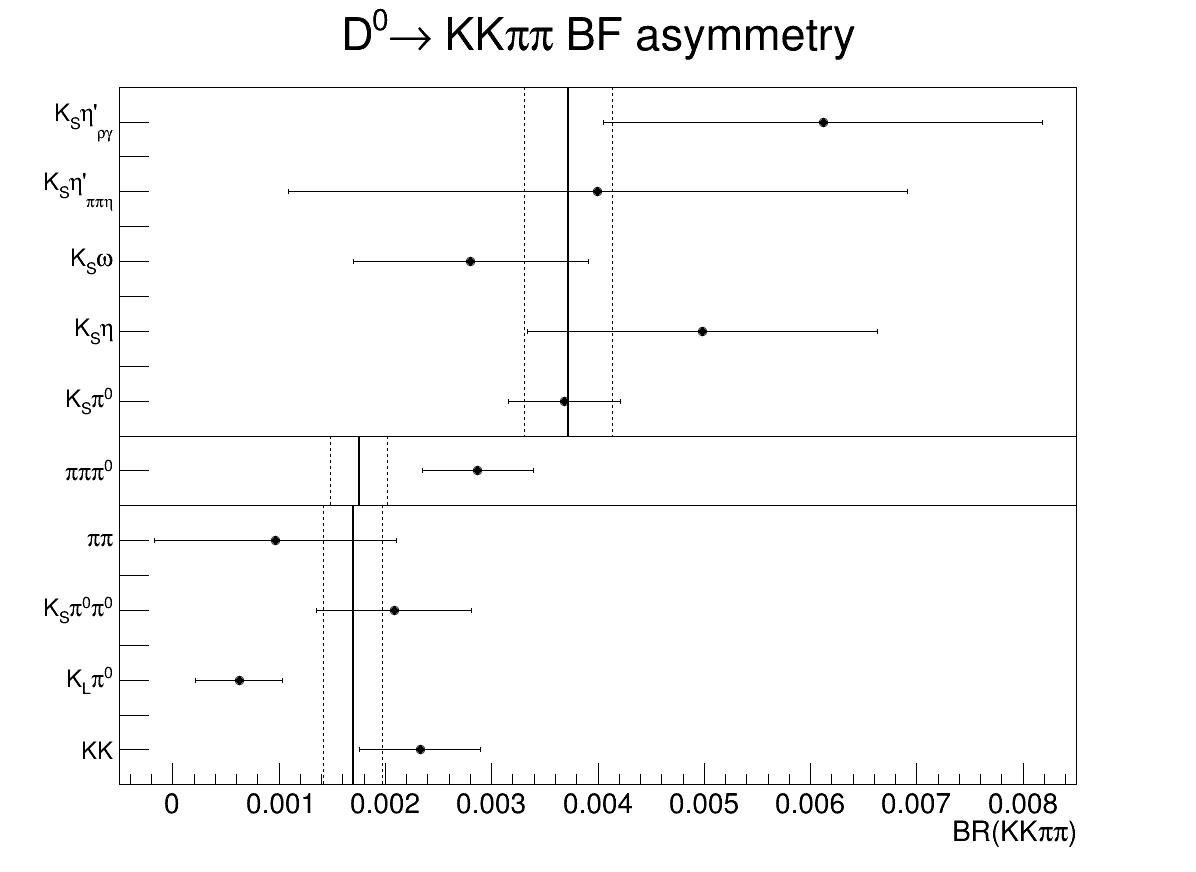
\includegraphics[width = 0.85\textwidth]{Plots/CPeven_fraction_combination_CPtags.png}
  \end{figure}
\end{frame}

\subsection{\texorpdfstring{$K_S\omega$}{KSomega} CP even tag using sPlot}

\begin{frame}{$K_S\omega$ CP even tag using sPlot}
  \begin{itemize}
    \setlength\itemsep{0.5em}
    \item{$D\to K_S\omega$ is CP even}
    \item{CP-even contamination from non-resonant $D\to K_S\pi\pi\pi^0$}
    \begin{itemize}
      \item{$F_+(K_S\pi\pi\pi^0) = 0.238\pm0.012\pm0.012$ from CLEO}
    \end{itemize}
  \end{itemize}
  \begin{figure}
    \centering
    \vspace{-0.2cm}
    \begin{subfigure}{0.40\textwidth}
      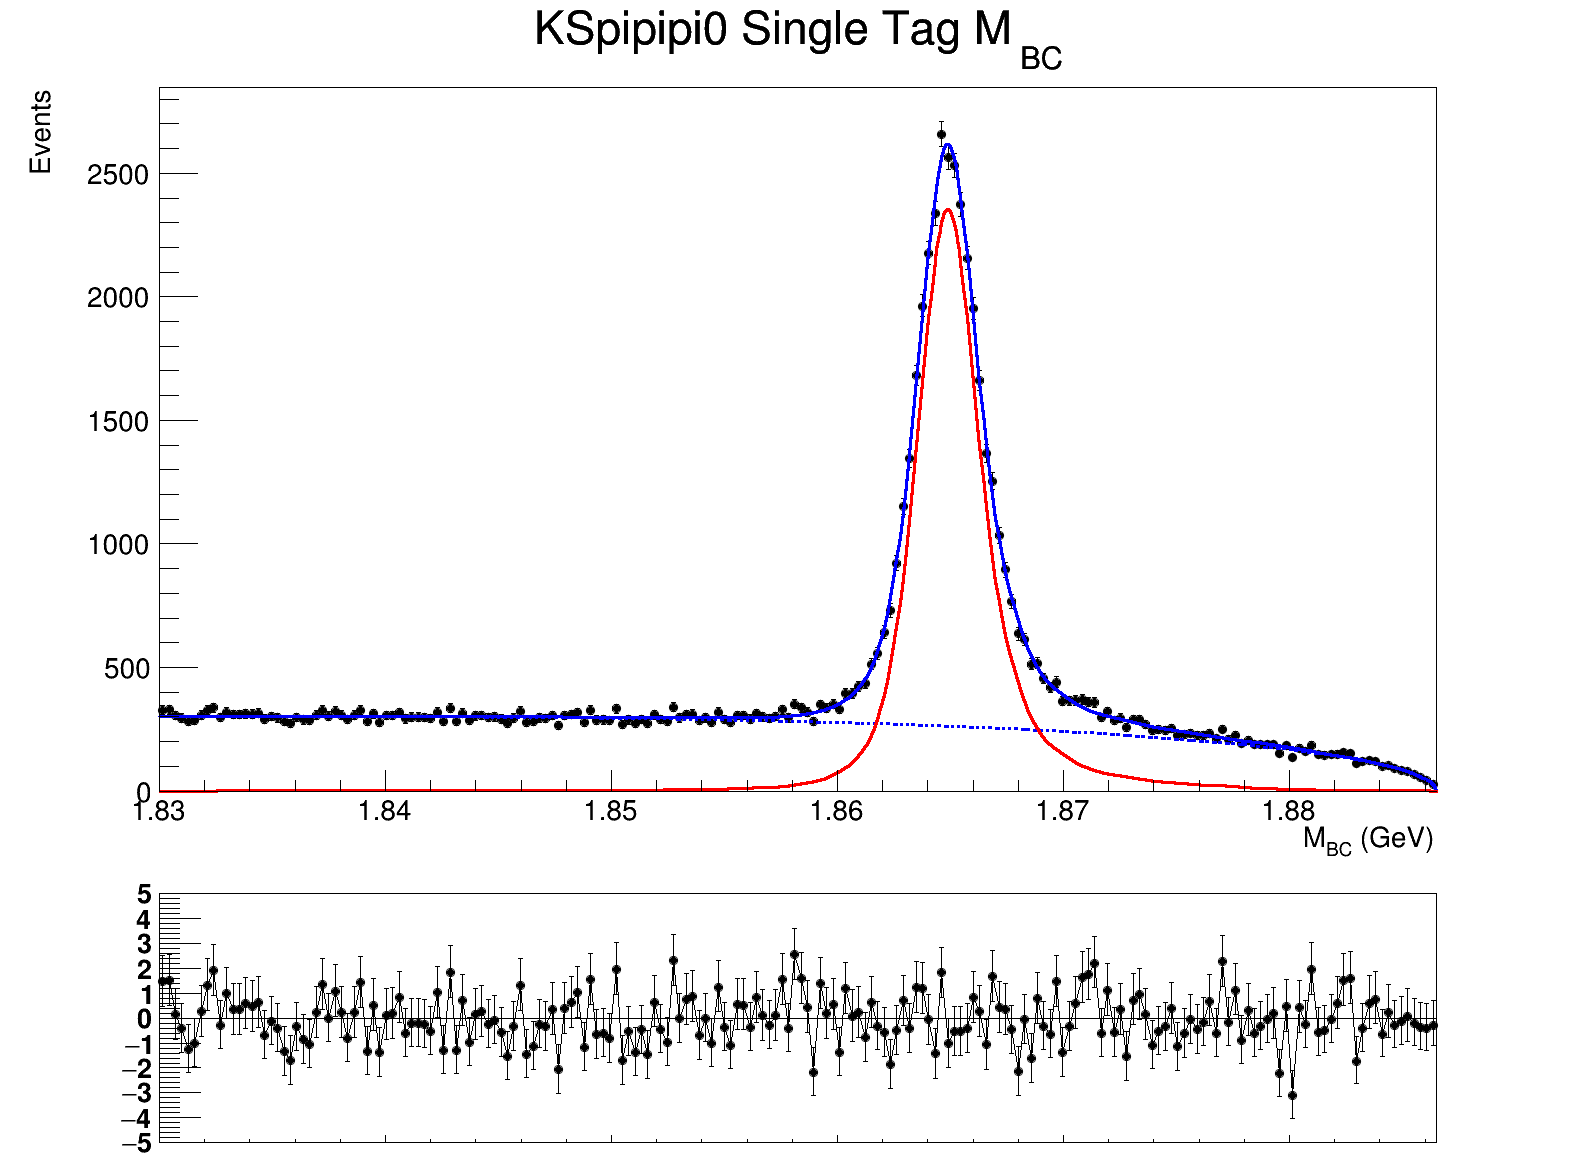
\includegraphics[width = 1.0\textwidth]{Plots/KSpipipi0_SingleTag_MBC_Plot.png}
      \caption{Single tag}
    \end{subfigure}%
    \begin{subfigure}{0.40\textwidth}
      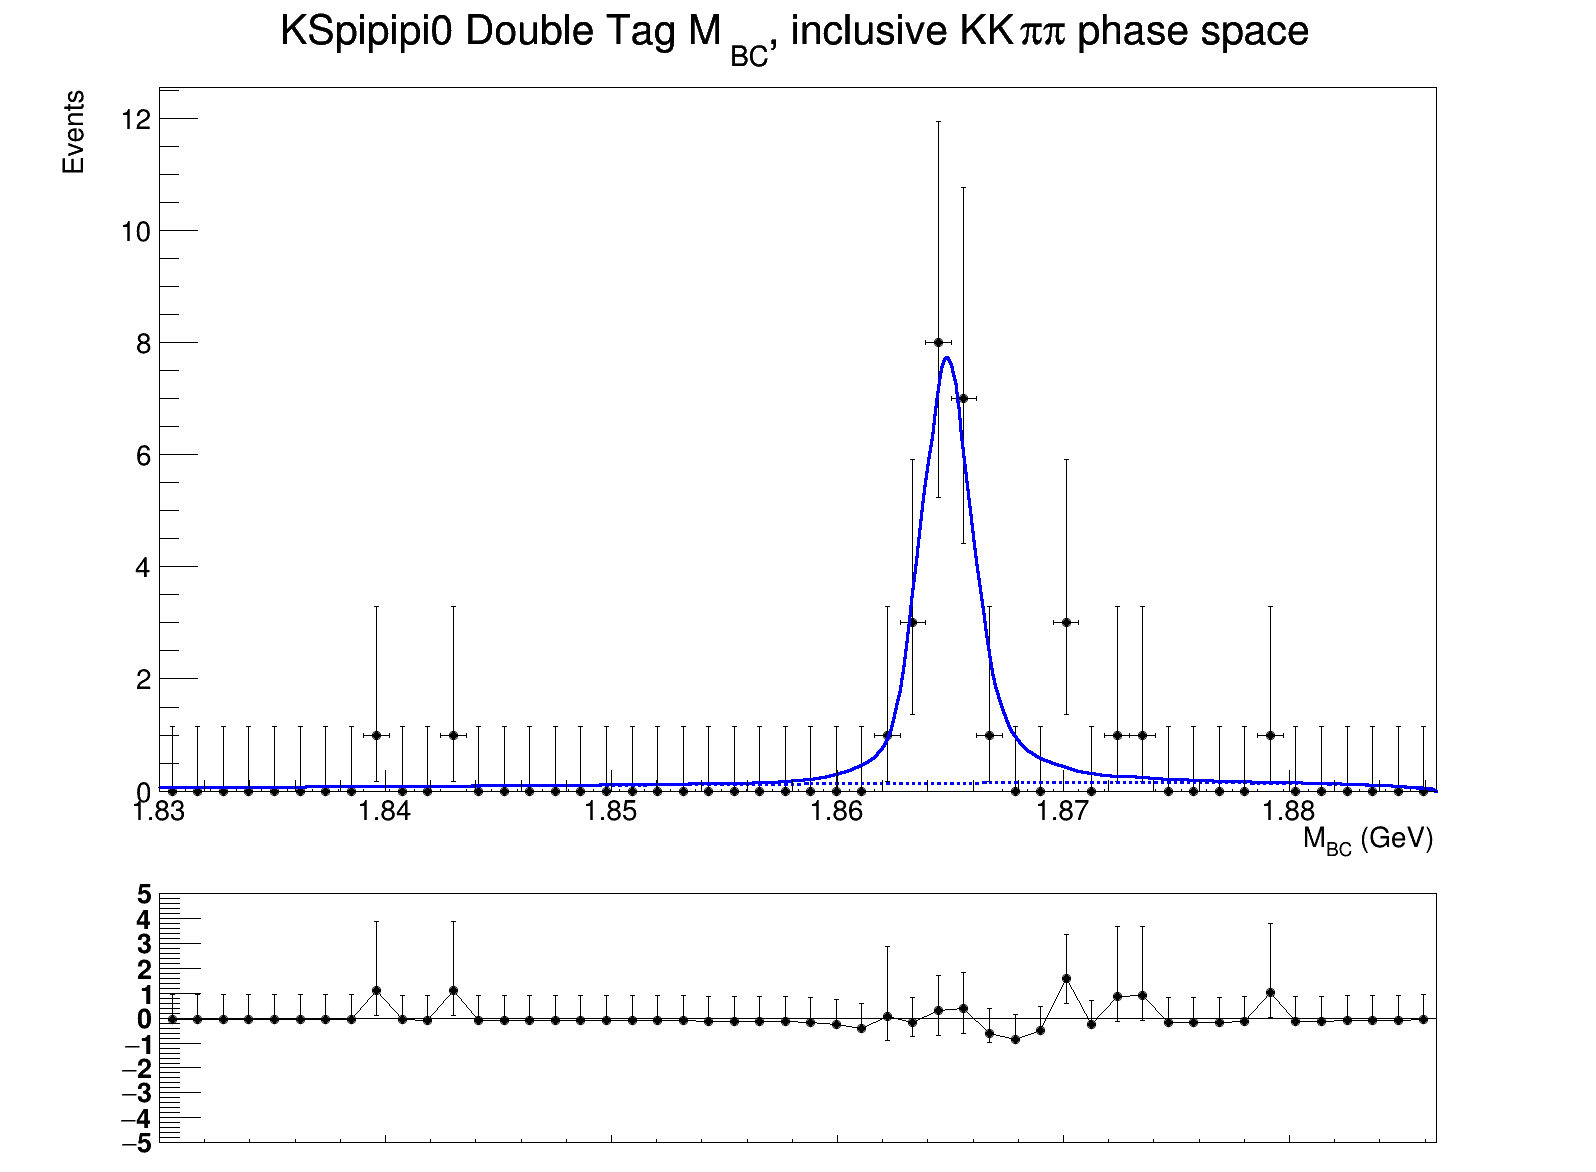
\includegraphics[width = 1.0\textwidth]{Plots/DoubleTagYield_DoubleTag_CP_KKpipi_vs_KSpipipi0_SignalBin0.png}
      \caption{Double tag}
    \end{subfigure}
    \caption{$D\to K_S\pi\pi\pi^0$ $D$ mass (beam constrained)}
  \end{figure}
\end{frame}

\begin{frame}{$K_S\omega$ CP even tag using sPlot}
  \begin{itemize}
    \item{Strategy:}
    \begin{enumerate}
      \item{From $D$ mass fit, remove non-$K_S\pi\pi\pi^0$ background using sPlot}
      \item{Fit $\pi\pi\pi^0$ invariant mass to obtain $K_S\omega$ yield}
    \end{enumerate}
  \end{itemize}
  \begin{figure}
    \centering
    \vspace{-0.2cm}
    \begin{subfigure}{0.40\textwidth}
      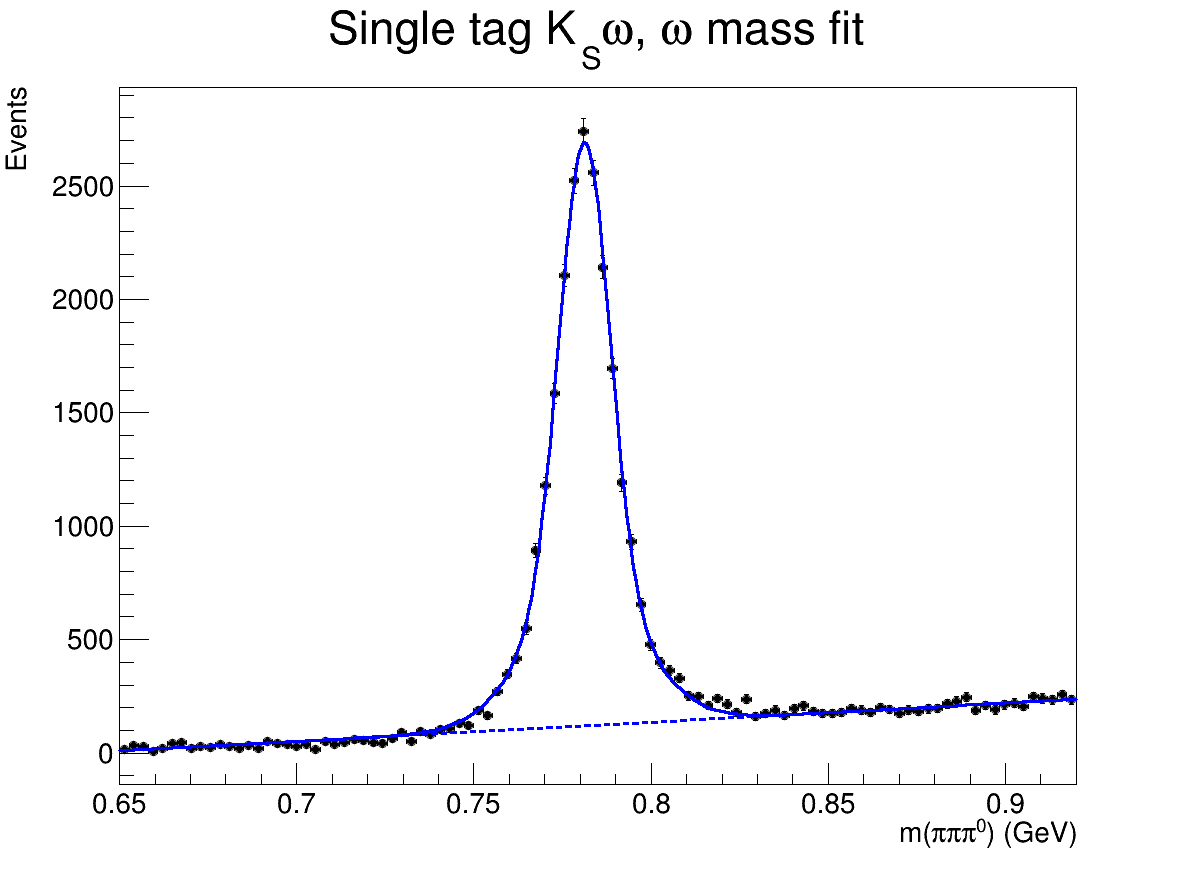
\includegraphics[width = 1.0\textwidth]{Plots/KSomega_ST_Mpipipi0.png}
      \caption{Single tag}
    \end{subfigure}%
    \begin{subfigure}{0.40\textwidth}
      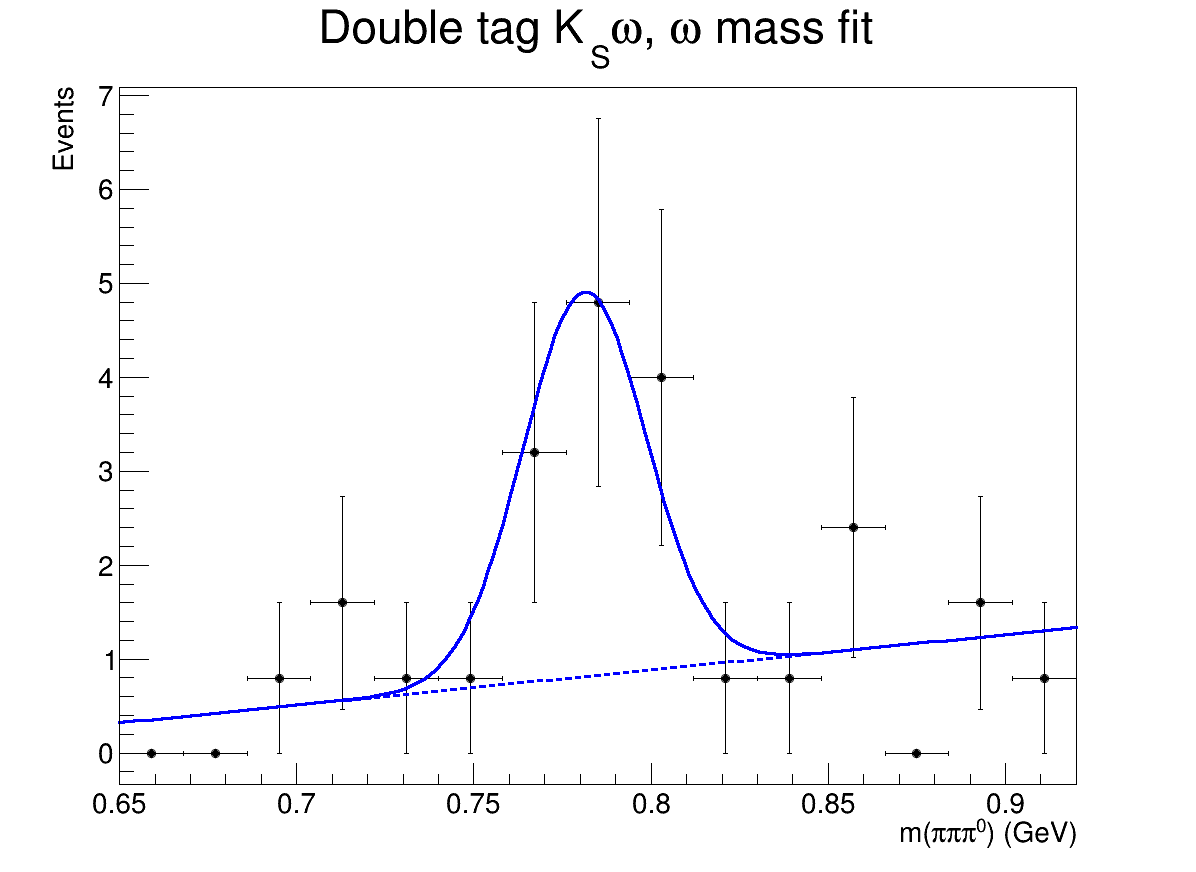
\includegraphics[width = 1.0\textwidth]{Plots/KSomega_DT_Mpipipi0.png}
      \caption{Double tag}
    \end{subfigure}
    \caption{$\pi\pi\pi^0$ invariant mass in $D\to K_S\pi\pi\pi^0$}
  \end{figure}
\end{frame}

\subsection{\texorpdfstring{$F_+$}{F+} measurement with \texorpdfstring{$K_S\pi\pi$}{KSpipi} tag}

\begin{frame}{$F_+$ measurement with $K_S\pi\pi$ tag}
  \begin{itemize}
    \item{With $K_S\pi\pi$, increase sensitivity through binning of $K_S\pi\pi$ phase space}
  \end{itemize}
  \begin{center}
    $M_i\propto\big(K_i + K_{-i} - 2\sqrt{K_iK_{-i}}c_i(2F_+ - 1)\big)$
  \end{center}
  \begin{itemize}
    \item{Problem: $KK\pi\pi$ reconstruction efficiency is too low $\to$ Low yields!}
  \end{itemize}
  \begin{figure}
    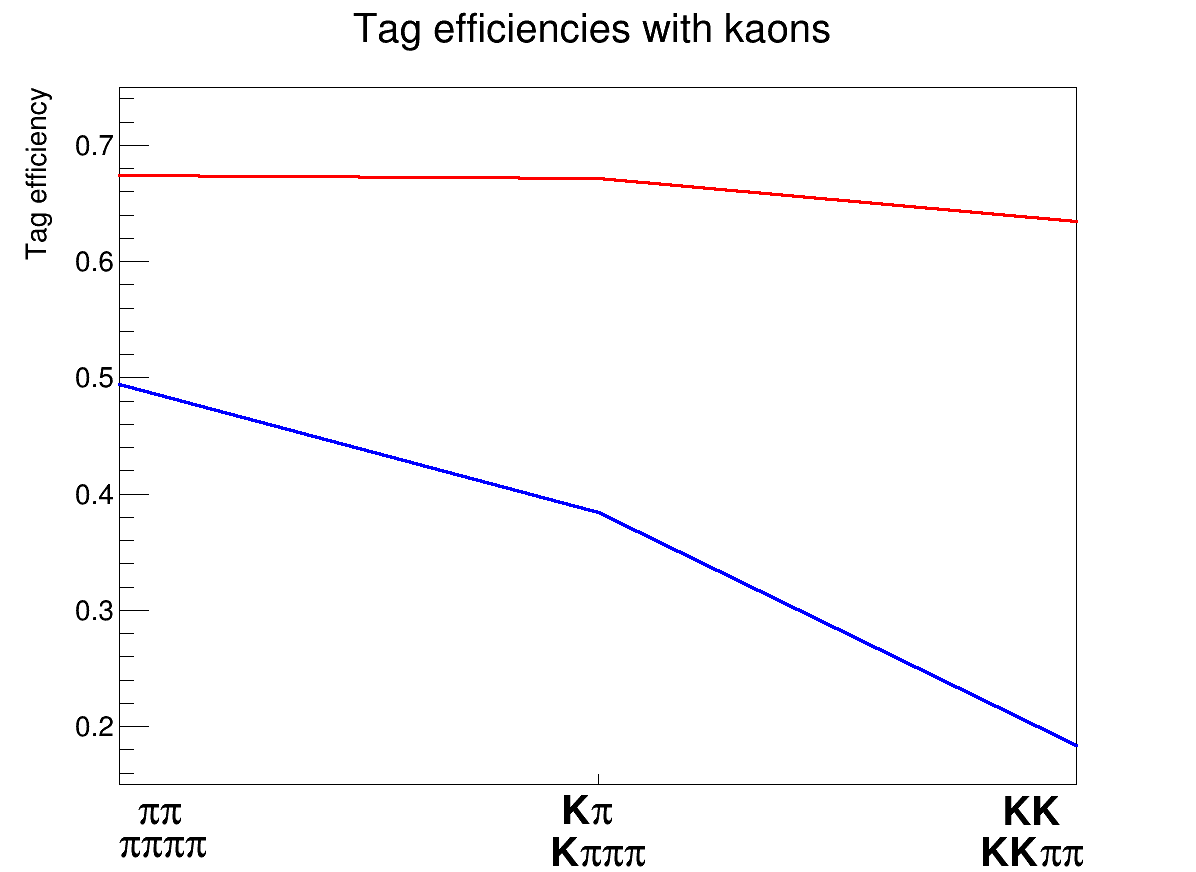
\includegraphics[width = 0.5\textwidth]{Plots/KaonTrackingEfficiency.png}
  \end{figure}
  \begin{itemize}
    \item{Likely explanation: Softer kaons $\to$ Kaons get stuck inside tracker}
  \end{itemize}
\end{frame}

\begin{frame}{$F_+$ measurement with $K_S\pi\pi$ tag}
  \begin{itemize}
    \setlength\itemsep{1.0em}
    \item{Solution: Partially reconstructed $KK\pi\pi$}
    \item{Strategy:}
    \begin{enumerate}
      \setlength\itemsep{0.5em}
      \item{Reconstruct $D\to K_S\pi\pi$}
      \item{Require 3 remaining good tracks consistent with $K\pi\pi$}
      \item{Use missing mass to reconstruct missing kaon}
    \end{enumerate}
  \end{itemize}
  \vspace{0.5cm}
  \def\arraystretch{1.2}%
  \begin{tabular}{l|c|c}
    Mode                                     & Inclusive yield & Double tag efficiency \\
    \hline
    $K_S\pi\pi$ (fully reconstructed)        & $67.2$          & $6.63 \pm 0.04$ \\
    $K_S\pi\pi$ (partially reconstructed)    & $85.9$          & $6.50 \pm 0.03$ \\
    $K_L\pi\pi$ (partially reconstructed)    & $176.9$         & $7.29 \pm 0.04$ \\
    \hline
  \end{tabular}
\end{frame}

\begin{frame}{Partially reconstructed $KK\pi\pi$ vs $K_S\pi\pi$}
  \begin{itemize}
    \item{Main challenge with partially reconstructed $KK\pi\pi$: $K\pi\pi\pi\pi^0$}
    \item{Require no $\pi^0$ candidates}
  \end{itemize}
  \begin{figure}
    \centering
    \vspace{-0.2cm}
    \begin{subfigure}{0.50\textwidth}
      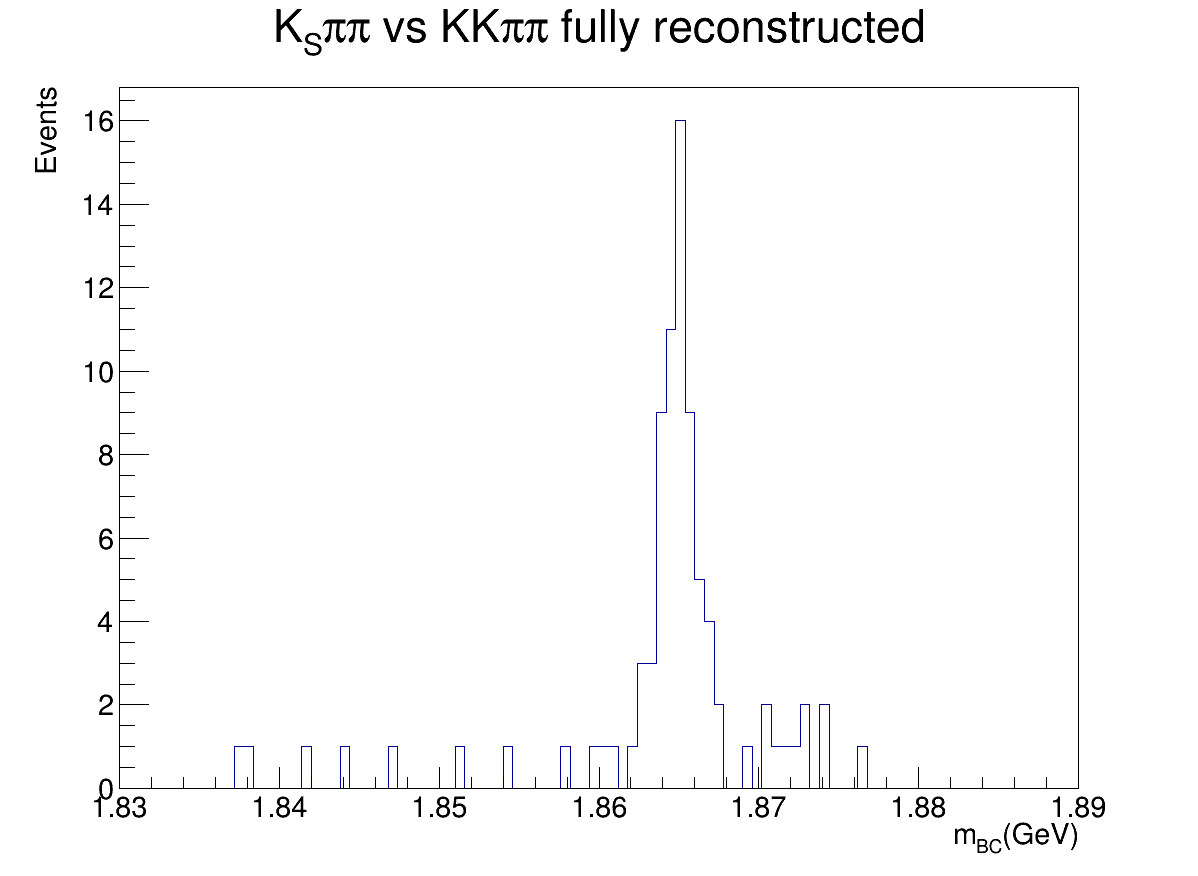
\includegraphics[width = 1.0\textwidth]{Plots/KKpipiVersusKSpipiMBC.png}
      \caption{Fully reconstructed}
    \end{subfigure}%
    \begin{subfigure}{0.50\textwidth}
      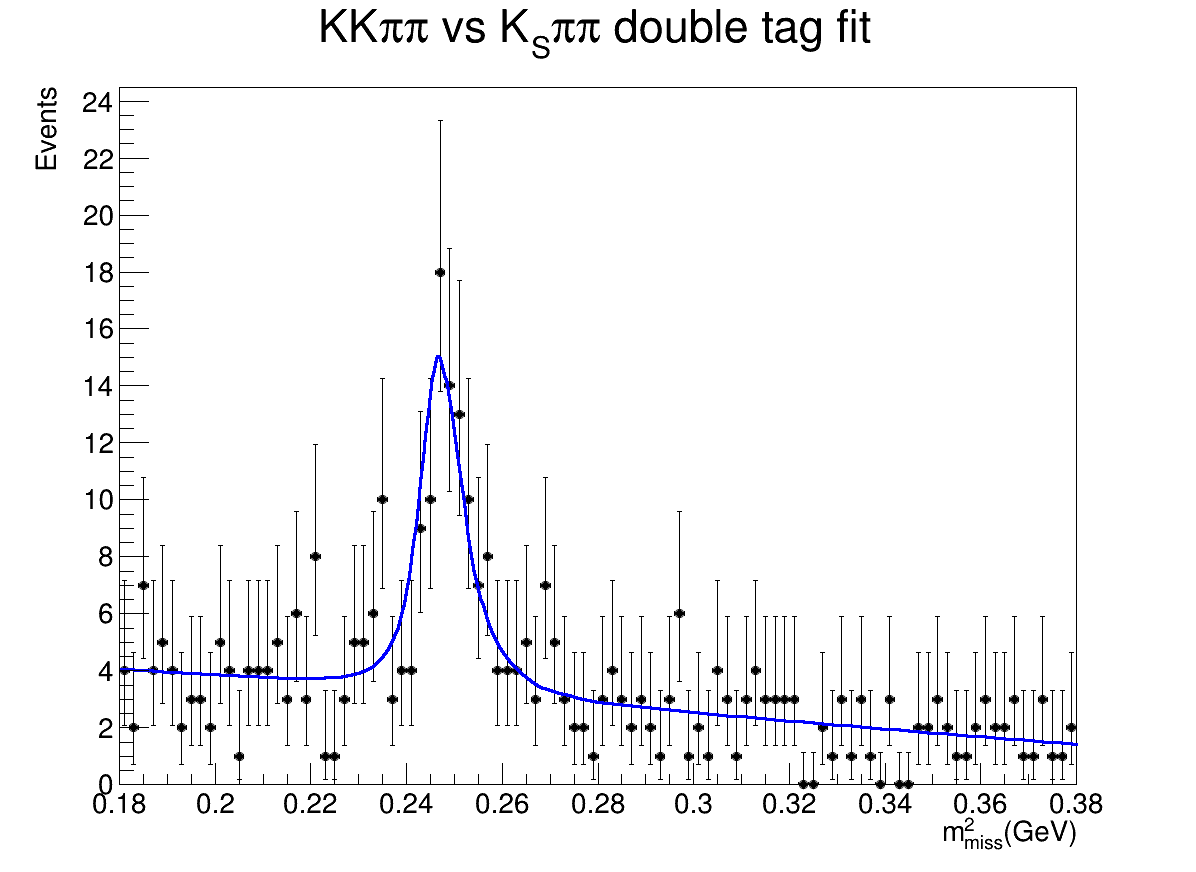
\includegraphics[width = 1.0\textwidth]{Plots/KSpipiPartReco_Inclusive_DoubleTagYield.png}
      \caption{Partially reconstructed}
    \end{subfigure}
    \caption{$KK\pi\pi$ vs $K_S\pi\pi$}
  \end{figure}
\end{frame}

\begin{frame}{$F_+$ measurement with $K_S\pi\pi$ tag}
  \begin{itemize}
    \item{Combine fully and partially reconstructed $KK\pi\pi$ vs $K_S\pi\pi$ to fit for $F_+$}
  \end{itemize}
  \begin{figure}
    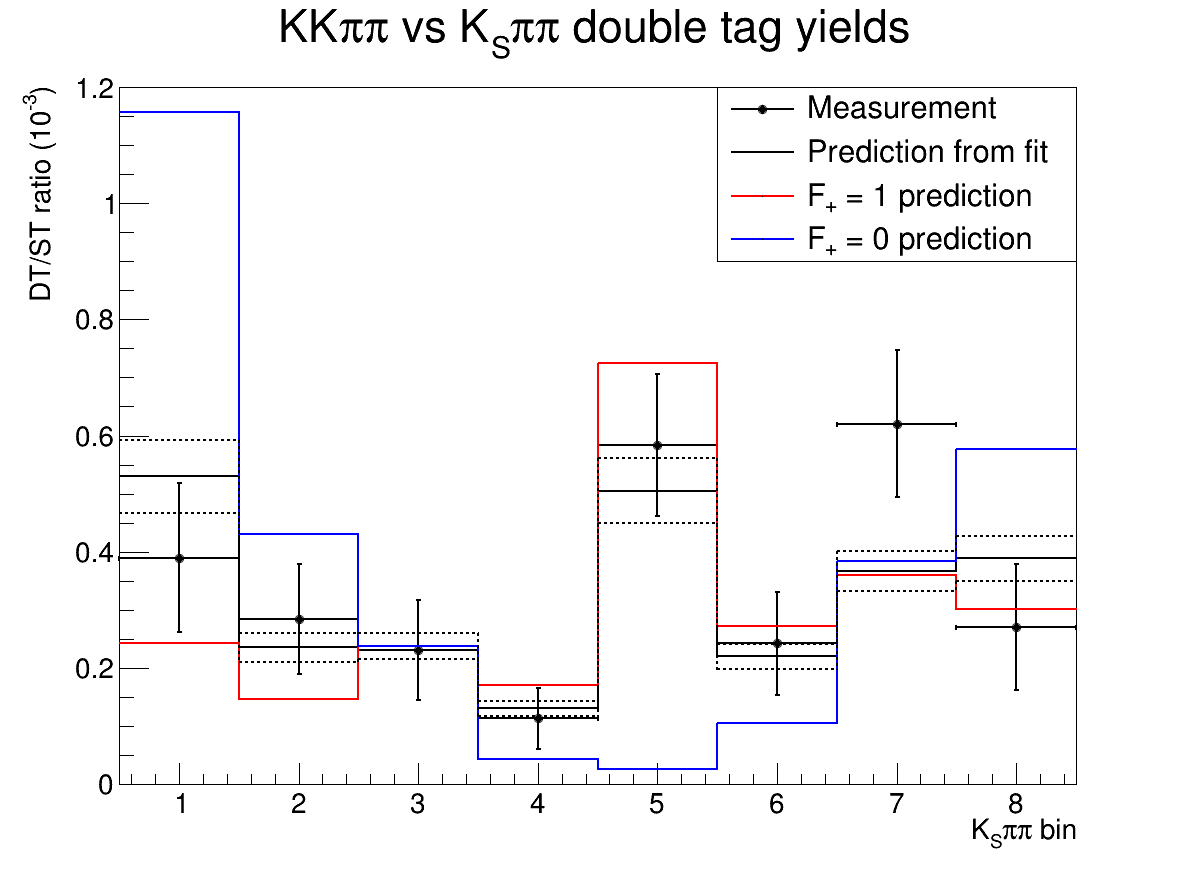
\includegraphics[width = 0.8\textwidth]{Plots/CPeven_fraction_combination_KSpipi.png}
  \end{figure}
\end{frame}

\begin{frame}{Combination of $F_+$ measurements}
  \begin{figure}
    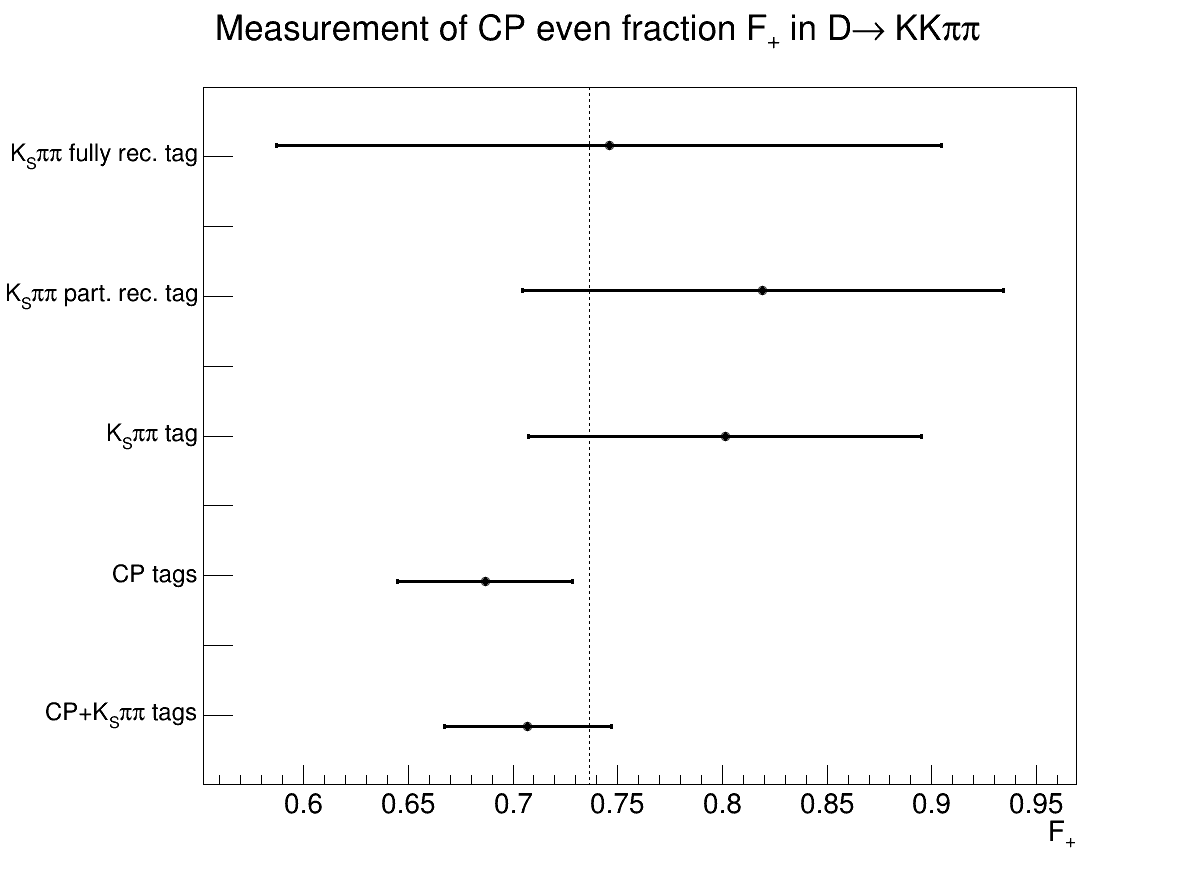
\includegraphics[width = 0.8\textwidth]{Plots/FPlus_combination_comparison.png}
  \end{figure}
\end{frame}

\begin{frame}{Next step: Include $K_L\pi\pi$ as well}
  \begin{itemize}
    \item{Irreducible background from $K_S\pi\pi$ with $K_S\to\pi^0\pi^0$}
    \item{$K_S\pi\pi$ has opposite quantum correlation which must be accounted for}
  \end{itemize}
  \begin{figure}
    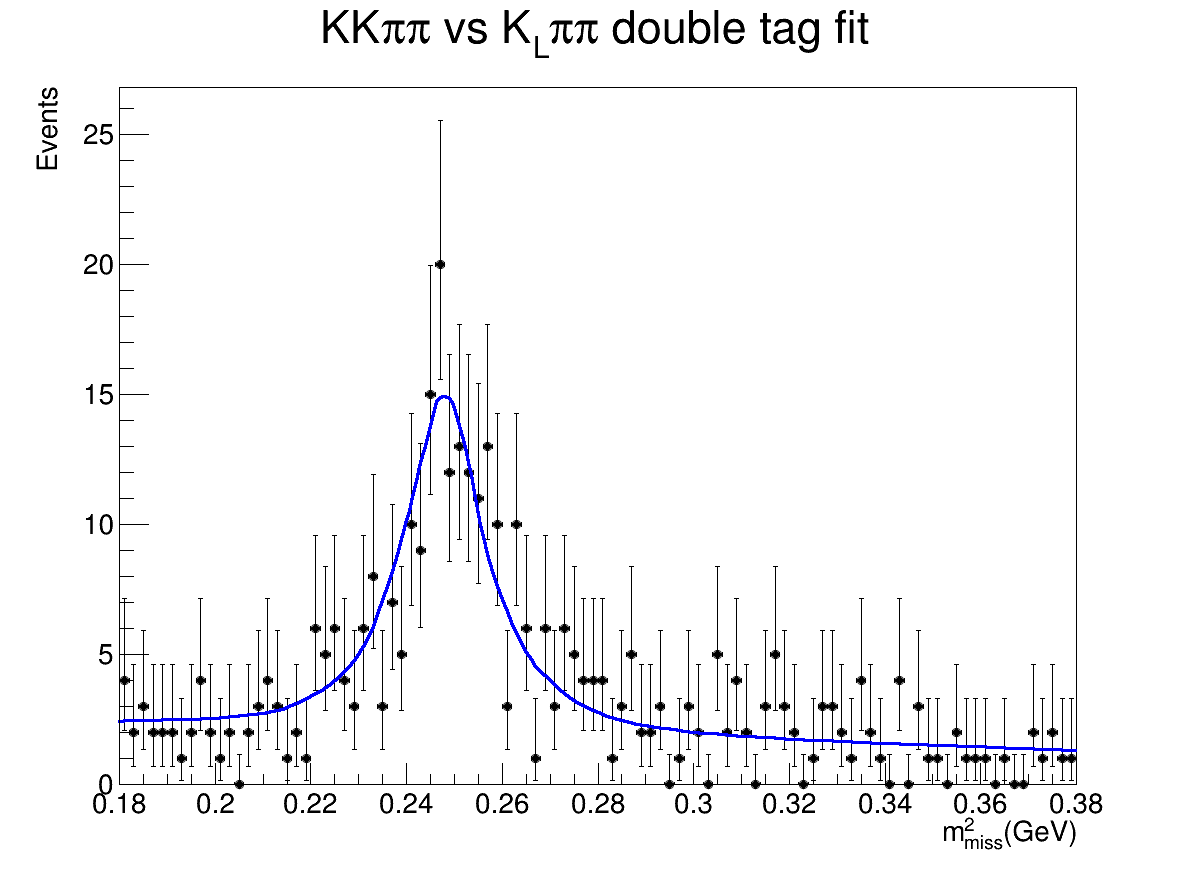
\includegraphics[width = 0.8\textwidth]{Plots/KLpipi_Inclusive_DoubleTagYield.png}
  \end{figure}
\end{frame}
  

\section{Summary}

\begin{frame}{Summary}
  \begin{itemize}
    \setlength\itemsep{1.5em}
    \item{LHCb $B^\pm\to(K^+K^-\pi^+\pi^-)_Dh^\pm$ GGSZ+GLW analysis:}
    \begin{itemize}
      \setlength\itemsep{0.5em}
      \item{2/3 reviewers have no further comments, waiting for final reply}
      \item{Sign of $s_i$ must be resolved}
    \end{itemize}
    \item{BESIII $D\to K^+K^-\pi^+\pi^-$ strong-phase analysis:}
    \begin{itemize}
      \setlength\itemsep{0.5em}
      \item{$K_S\omega$ tag added to $F_+$ combination using sPlot}
      \item{Partially reconstructed $KK\pi\pi$ vs $K_S\pi\pi$ shows promising results}
      \item{$F_+$ measurement performed in $KK\pi\pi$ vs $K_S\pi\pi$ binned analysis}
      \item{Next steps:}
      \begin{itemize}
        \item{Perform $F_+$ measurement with $K_L\pi\pi$}
        \item{Add CP tags $K_L\pi^0\pi^0$, $K_L\omega$ to $F_+$ combination}
      \end{itemize}
    \end{itemize}
  \end{itemize}
  \begin{center}
    \huge Thank you!
  \end{center}
\end{frame}

\end{document}
